\chapter{Attack Model from Digital Signature}

\begin{flushleft}
    Definiamo per prima cosa la \textbf{superficie di attacco} e le \textbf{conoscenze} dell'avversario, in questo caso, sono le di coppie (\textit{message}, \textit{signature}) a cui ha accesso l'attaccante (definendo il tipo di messaggio). \\
    Lo \textbf{scopo} dell'attaccante è quello di \textbf{\textit{forgiare}} una coppia valida (\textit{message}, \textit{signature}) per un certo messaggio.

    \smallskip

    \textbf{Nota}: un obiettivo implicito è quello di risalire alla \textbf{chiave segreta}, obiettivo per qualunque schema a chiave segreta (privata o simmetrica), ma per gli schemi di firma digitali una progettazione sbagliata potrebbe renderli più vulnerabili a \textbf{\textit{key recovery attacks}}.

    \smallskip

    Partiamo dal definire i possibili modelli di attaccante classificati in base alla \textbf{\textit{attack surface}}:

    {\centering
        \begin{minipage}[c]{0.75\textwidth}
            \begin{itemize}[nosep]
                \item \textbf{\textit{No message}}: l'attaccante non ha accesso a nessuna coppia $(m, s)$.
                \item \textbf{\textit{Random message}}: l'attaccante conosce una lista di coppie $[(m, s)]$ per messaggi randomici.
                \item \textbf{\textit{Known message}}: l'attaccante può estrarre una qualunque lista $[(m, s)]$ prima di conoscere la chiave pubblica.
                \item \textbf{\textit{Chosen message - Chosen Message Attack (CMA)}}: l'attaccante può estrarre una qualunque lista $[(m, s)]$ dopo che gli è stata rivelata la chiave pubblica.
            \end{itemize}
        \end{minipage}
        \hfill
        \begin{minipage}[c]{0.1\textwidth}
            \centering
            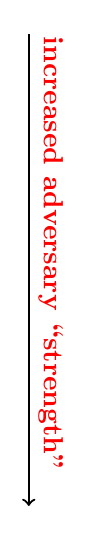
\begin{tikzpicture}[scale=1]
                \node[rotate=270, anchor=south, text=red] at (0,2.2) {\textbf{increased adversary ``strength''}};
                \draw[<-, thick, black] (0,-1.0) -- (0,5.0);
            \end{tikzpicture}
        \end{minipage}
    \par}
    
    \newpage

    Consideriamo ora i possibili modelli di attaccante in base al \textbf{tipo di compromissione} che possono effettuare:

    {\centering
        \begin{minipage}[c]{0.75\textwidth}
            \begin{itemize}[nosep]
                \item \textbf{\textit{Key Recovery}}: riesce a \textit{forgiare} una qualunque coppia $(m, s)$.
                \item \textbf{\textit{Forging valid couples $(m, s)$}}
                \begin{itemize}[nosep]
                    \item \textbf{\textit{selective}}: può \textit{forgiare} alcune coppie $(m, s)$.
                    \item \textbf{\textit{existential message forgery}}: definita \textbf{\textit{weak}} se riesce a forgiare almeno una volta una coppia $(m, s)$ per ogni messaggio $m$ per il quale non è stata fatta una precedente \textit{signature} $s$. \textbf{\textit{strong}}, invece, se riesce a forgiare almeno una coppia $(m, s)$ per qualunque messaggio.
                \end{itemize}
                \item \textbf{\textit{Key substitution}}: può verificare una coppia $(m, s)$ per due chiavi pubbliche diverse
            \end{itemize}
        \end{minipage}
        \hfill
        \begin{minipage}[c]{0.1\textwidth}
            \centering
            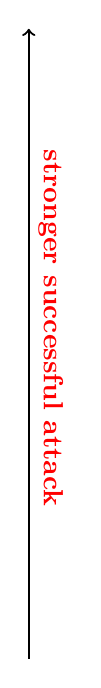
\begin{tikzpicture}[scale=1]
                \node[rotate=270, anchor=south, text=red] at (0,2.2) {\textbf{stronger successful attack}};
                \draw[->, thick, black] (0,-2.0) -- (0,6.0);
            \end{tikzpicture}
        \end{minipage}
    \par}
    
    \medskip

    \textcolor{red}{\textbf{\textit{``Standard'' security guarantees of Digital Signature}}}: in questo caso vengono rappresentati i termini di sicurezza in base a cosa l'avversario non è capace di fare, \textit{signature scheme} sono sicuri se garantiscono \textbf{\textit{UnForgeability (UF)}}.

    \smallskip

    \textbf{\textit{Standard Digital Signature}} devono almeno raggiungere \textbf{EUF-CMA} ovvero \textbf{\textit{Existential UnForgeability Under Chosen Message Attack}}, ma in alcuni scenari non basta, e quindi viene richiesto \textbf{SUF-CMA} ovvero \textbf{\textit{strong} EUF-CMA}, quindi dato $(m, s)$ per qualunque $m$, l'avversario non può calcolare $s'$ tale per cui la coppia $(m, s')$ è una coppia valida. \\
    \textbf{Nota}: ``debole'' è implicitamente sotto garanzie di \textbf{EUF-CMA}.
\end{flushleft}